\documentclass[11pt,a4paper]{article}

\usepackage{amsmath}  
\usepackage{amsfonts} 
\usepackage{graphicx}
\graphicspath{ {./images/} }
%\usepackage[demo]{graphicx}
\usepackage[usenames]{color}
\usepackage{mathtools}
\usepackage{algorithm}
\usepackage[noend]{algpseudocode}
\usepackage{float}
\usepackage{xcolor}


\DeclarePairedDelimiter{\abs}{\lvert}{\rvert}
\DeclareMathOperator{\esssupp}{ess\,supp}


 \textwidth=16cm \hoffset = -1.9cm
 \lineskip=1.5\lineskip


% MATH -----------------------------------------------------------
\newcommand{\Real}{\mathbb R}
\newcommand{\eps}{\varepsilon}
\newcommand{\diag}{\mathrm{diag}}
\newcommand{\nbr}{\mathrm{nbr}}
\newcommand{\F}{\mathcal{F}}
\newcommand{\Hil}{\mathscr{H}}
\newcommand{\LL}{\mathcal{L}}
\newcommand{\G}{\mathscr{G}}
\newcommand{\s}{\mathbb{S}}
\newcommand{\p}{\mathscr{P}}
\newcommand{\C}{\mathscr{C}}
\newcommand{\one}[1]{\mathbf{1}_{\{#1\}}}
\newcommand{\oneset}[1]{\mathbf{1}_{#1}}
\renewcommand{\P}{\mathbb{P}}
\newcommand{\Q}{\mathsf{Q}}
\newcommand{\E}{\mathbb{E}}
\newcommand{\osimplex}{\mathcal{S}^{d-1}}
\newcommand{\csimplex}{\bar{\mathcal{S}}^{d-1}}
\newcommand{\argmin}{\mathrm{argmin}}
\newcommand{\argmax}{\mathrm{argmax}}
\newcommand{\var}{\mathrm{Var}}
\newcommand{\cov}{\mathrm{Cov}}
\newcommand{\ind}{\mathrm{I}}
\newcommand{\D}{\mathscr{D}}
\newcommand{\Borel}{\mathscr{B}}
\newcommand{\M}{\mathcal{M}}
\newcommand{\Z}{\mathcal{Z}}
\renewcommand{\d}[1]{\ensuremath{\operatorname{d}\!{#1}}}

\newcommand{\ben}{\begin{enumerate}}
\newcommand{\een}{\end{enumerate}}
\newcommand{\ds}{\displaystyle}

\DeclareMathOperator{\trace}{tr}
\DeclareMathOperator*{\esssup}{ess~sup}
\DeclareMathOperator*{\essinf}{ess~inf}
\DeclareMathOperator*{\diam}{diam}
\DeclareMathOperator*{\ROC}{ROC}
\DeclareMathOperator*{\sinc}{sinc}
\DeclareMathOperator*{\sign}{sign}
\newcommand{\voila}{\hfill $\blacksquare$}
\newcommand{\Id}{\mathrm{Id}}
\newcommand{\K}{\mathbb{K}}
\renewcommand{\Re}{\mathrm{Re}}
\renewcommand{\vec}[1]{\mathbf{#1}}
\newcommand*\diff{\mathop{}\!\mathrm{d}}




\title{New Sequential Importance Sampling methodology applied to a spatial-temporal point process model for the Red Imported Fire Ants invasion in Queensland Australia}

\begin{document}
\maketitle
{\color{red}
\section{Abstract}\label{section:abstract}
We present an application of a new Sequential Importance Sampling methodology to one of the world's 100 worst invaders: the Red Imported Fire Ant (RIFA). (to be continued ...)}

{\color{red}
\section{Introduction}\label{section:introduction}
The Red Imported Fire Ant \textit{Solenopsys Invicta} Buren \cite{GISD} or RIFA is native to South America and has spread globally \cite{Wetterer} negatively impacting human health, public safety, ecosystems and agriculture. Distribution currently includes the United States, Australia, New Zealand, China, Malaysia, Singapore and the West Indies \cite{Wang} \cite{GISD}. In Australia it has been introduced in seven locations over the period 2001-2016 \cite{WylieMay16}, and while the National Red Imported Fire Ant Eradication Program elminiated six of these incursions, the remaining one originated in Brisbane had a ``footprint" 4,000 $\text{km}^2$ in 2015. The eradication program successfully managed to reduce the spread of the invasion which otherwise would have been estimated to cover an area of 48,000 $\text{km}^2$ \cite{Wylie2020}. However, a complete eradication has not yet been achieved. Complete eradication of an invasive species is usually hard and the success of an eradication program will depend on many factors including how early the first detection of the invasion occurred. When large areas are potentially infested and surveillance is required to determine where to apply treatment, eradication can take years. Some areas that might be infested are not regularly surveyed owing to the high cost of monitoring, and some individuals in surveyed locations are missed because surveillance methods are imperfect \cite{Royle} therefore observations are “incomplete”. These two factors create uncertainty about whether eradication efforts will succeed  \cite{Keith}. Understanding and correctly modelling the true extension of an invasion is fundamental to evaluate correctly how successful an eradication program is and whether to continue with current eradication methods. 

Our new Sequential Importance Sample strategy aim to assess the current extent of an invasion imputing missing data in the presence of incomplete observations made sequentially in time. After receiving data regarding the location of some of the nests, we simulate the locations of the unknown number of undetected colonies. When new observations are made our simulations can be improved by these new observations. In order to do so we propose a two-step iterative process in which states of the system are alternatively simulated in accordance with past observations, then corrected in light of the newly received observations. As is typical of SIS methods we generate a population of particles, each representing a plausible sequence of system states, and we evolve each particle at each time step according to a model of system dynamics. when new observations arrive in real time we use these observations to adjust the weights assigned to particles. The crucial new element in our method is that we allow missing values imputed at earlier time steps to be corrected improving the quality of our estimation for the entire history of the invasion.

We model the fire ants invasion as a self-exciting Spatial-temporal point process.  (to be continued ...)}


\section{The Model}\label{section:model}

We are proposing a new model for the RIFA invasion based on a self-exciting point process.

In this new approach we are seeking to simplify and improve on Keith and Spring agent-based model \cite{Keith} with the aim to reduce the running time without compromising on flexibility and completeness.

The model of Keith and Spring focused on reconstructing the historical trajectory of the invasion to determine if the current eradication strategy was successful. Their method consisted of constructing a likelihood model in terms of some unknown parameters that included, among other things, the phylogeny, jump type, founding type and treatment success rate. They then constructed the dependencies among the known and unknown parameters and defined all conditional distributions.

The posterior distribution was then sampled using a generalised Gibbs technique that enables transdimensional sampling, which is used when the number of parameters is unknown, as in their case.

A key feature of our model is that it will not need to include the phylogeny of the nests in the likelihood, which will result in a much lower computational time when running the inference code. This will also allow the model to be adapted to other type of problems where control strategies will have to be decided rapidly as new data is acquired. {\color{red}The phylogeny can however can be reconstructed if needed}.

In our model we consider the detection processes in parallel with the founding events in a similar way as in Jewell's model for infectious diseases \cite{Jewell}. We then included unobserved nests alongside observed nests in the detection likelihood to fully model the missing data.

Let us consider a self-exciting spatial-temporal point process $N$ as a generalization of an Hawkes model {\color{red} \cite{Hawkes71}}. We can then specify an intensity function $\lambda(x, y, t)$ which represents the infinitesimal expected  rate of events at time $t$ and location $(x, y)$  given all the events up to time $t$.

Here $\mathcal{F}$ is a $\sigma$-algebra on $S \times [0, \infty )$, where $S$ is a bounded region of $\mathbb{R}^2$ and $[0, \infty)$ is the time interval. $N(A)$ is a counting measure $N: \mathcal{F} \to \mathbb{R}$ representing the number of points in $A$ for $A \in \mathcal{F}$.

We will consider $N$ to be an inhomogeneous Poisson process, for which $\lambda(x, y, f)$ is deterministic, i.e. depends only on $(x, y)$ and $f$ \cite{Shoenberg} {\color{red}VVV I am not sure this is correct. If N is a Poison process and $\lambda$ is deterministic we would not have a self exciting point process which depends on the history of all events up to time $t$. I think it is the background process that is a Poisson process with rate $\mu$ and it is the likelihood of the process that is that of an inhomogeneous Poisson process while N is a random counting measure (a stationary point process)}. The function $g(x - x', y - y', f - f')$ is the clustering density, where $f'$ are the times of founding of parents nests and the spatial coordinates $(x', y')$ will specify the location $s'$ of a parent nest.

We can then write the intensity function for new nests, {\color{red} conditional over the past history of the process $\mathcal{H}_t$}, in term of a stochastic integral:

\begin{equation}\label{eq:intensity}
    \lambda(x, y, f {\color{red}| \mathcal{H}_f}) = \mu(x, y, f) + \int_{0}^{f} \iint_{S} g(x - x', y - y', f - f') \d N(x', y', f')
\end{equation}
were $\d N(x', y', f') = 1$ if the infinitesimal element $\d N(x', y', f')$ contains a parent and is 0 otherwise. $\lambda(x, y, t)$ may be thought of as the frequency with which events are expected to occur around a particular location $(x, y, t)$ in space–time.

In our model the temporal behavior of the process is independent of the spatial behavior so we can write

\begin{equation*}
    \lambda(x, y, f {\color{red}| \mathcal{H}_f}) = \mu(x, y, f) + \int_{0}^{f} \iint_{S} q(f-f') l\Big((x - x'), (y - y')\Big) \d N(x', y', f')
\end{equation*}
where $m$ and $l$ are the triggering functions for time and space respectively. {\color{red} From now on we will omit the explicit conditioning on the past history $\mathcal{H}_f$ for ease of notation.}

New individuals from the invasive species can be introduced at any time by carriers like animals or humans. For simplicity, in the RIFA invasion we will assume that there are no exogenous introductions and we will therefore set the background term $\mu(x, y, f) $ equal to 0.

{\color{red} Since N is a counting measure, we can write equation (\ref{eq:intensity}) as

\begin{equation*}
    \lambda(x, y, f) = \sum_{ p: f_p < f } q(f - f_p) l \Big((x - x_p),(y - y_p) \Big)
\end{equation*}
where the sum is over all the $p$ parent nests $(x_p, y_p, f_p)$ with $t_p < t$.}

Each parent nest will be able to found more than one nest, with the number of nests founded per nest per month being a parameter $\zeta$, therefore the temporal triggering kernel will be a step function. Also the nests will have a maturation time $t_m$ of 8 months, meaning that before this time they will not be able to produce new nests. 

The step function will be:

\begin{equation*}
    q (f - f_p | \zeta) =
    \begin{cases}
        0, & \mbox{if} \quad f - f_p < t_{m} \\
        \zeta, & \mbox{if} \quad f - f_p \geq t_{m}
    \end{cases}
\end{equation*}
where $f$ is the founding time of the new nest and $f_p$ is the founding time of the parent nest.

{\color{red} Biological invasions spread through local movements and by long-distance jumps \cite{Suarez}. The long distance jumps are often human-assisted and create new clusters far from the founding cluster. We will therefore consider two unknown founding types: a local founding event with $U_i = 0$ and the long-distance jump with $U_i = 1$. The vector of jump type is therefore $U = (U_1, \dots, U_N)$ with $N$ the total number of founded nests.

The vector of jumps types will have probability density function

\begin{equation*}
    p(U| \gamma ) = 2{N \choose \nu}(\gamma)^{2\nu}(1 - \gamma)^{2(N - \nu)}
\end{equation*}
where $\gamma$ is the probability of a long jump and $\nu$ is the number of long-distance jumps.}

For the newly founded nests we will consider a radial distance from the parent nest with an exponential distribution for the local founding event and a {\color{red}l\'evy distribution for the long-distance jumps}. The distribution over the angular direction will be uniform as it is equally possible to found a nest in every direction from the parent nest. {\color{red} Therefore the probability distributions for the short jumps $l_0$ and for the long jumps $l_1$ will be

\begin{equation*}
    l_0\Big((x - x_p), (y - y_p) | U, \sigma \Big)= J \bigg(\frac{1}{2 \pi} \sigma e^{- \sigma r}\bigg)
\end{equation*}

\begin{equation*}
    l_1\Big((x - x_p), (y - y_p) | U, c \Big)= J \bigg(\frac{1}{2 \pi} \sqrt{\frac{c}{2 \pi}} \frac{e^{- \frac{c}{ 2 r}}}{r^{3/2}}\bigg)
\end{equation*}}
where $J$ is the Jacobian and $r$ is the radial distance between the parents nests and the newly founded nests.

We also make the assumption that nests are killed as soon as they are detected, so we introduce an indicator function $I(t_d - t)$ such that

\begin{equation*}
    I (t_d - t) =
    \begin{cases}
        1, & \mbox{if} \quad t_d -  t> 0 \\
        0, & \mbox{otherwise}
    \end{cases}
\end{equation*}
where $t_d$ represents the time of detection. So the conditional intensity function will be

\begin{equation*}
    \lambda(x, y, t, f) = \sum_{p:f_p < f} q(f - f_p | \zeta) I(t_d - t)\cdot p(U | \gamma) l_0(x, y | U, \sigma) l_1(x, y | U, c)
\end{equation*}
{\color{red} where we must have that $f_p\leq t_d$. Notice that this process is Markovian.

As demonstrated by Hawkes and Oakes \cite{Hawkes74}, any stationary self-exciting point process with finite intensity may be interpreted as a Poisson cluster process with the number of offspring for each event drawn from a Poisson distribution with mean 

\begin{equation} \label{eq:NumOffsp}
    m = \int_0^T \iint_S g(x-x', y-y', f-f')\d N(x', y', f').
\end{equation}}
The likelihood at time $T$, {\color{red}as the probability density function of a set of observed nests for the given parameters,} will then be that of an inhomogeneous Poisson process for the founding process with intensity $\lambda(x, y, t)$ {\color{red} (See Reinhart \cite{Reinhart} for a derivation of the likelihood for self-exciting spatial-temporal point processes).}

We will consider the time from establishment to notification $(t_i - f_i)$ of an offspring nest $i$ as a random variable exponentially distributed with parameter $\varphi$

\begin{equation*}
    h(t_{i} - f_{i} | \varphi) = \varphi \exp (- \varphi(t_{i} - f_{i})).
\end{equation*}
The Likelihood for a set of $n$ locations $(s_{1}, ... , s_{n})$ with $s_i = (x_i, y_i)$, founding times $f_{1}, ... , f_{n}$, and detection times $(t_{1},  ... , t_{n})$ will then be:

\begin{equation*}
    \begin{aligned}
        L(s_{1}, ..., s_{n}, f_{1}, ..., f_{n}, t_{1}, ..., t_{n} ; \Theta) = & \Bigg[ \prod_{i = 1}^{n} \lambda(s_{i}, t_{i}, f_{i}) \Bigg] \exp \Bigg(- \int_{0}^{T} \int_{0}^{T} \int_{S} \lambda(s, t, f) \d s \d t \d f \Bigg) \\ 
        & \prod_{\{ i : t_{i} < T \} } h(t_{i} - f_{i}) \prod_{ \{ i : t_{i} = \infty \} } \int_{T}^{\infty} h(t - f_{i}) \d t
    \end{aligned}
\end{equation*}
where $t_{i} = \infty$ if nest $i$ has not been detected at time $T$ and where $n$ is the number of nests founded. The quantity $h(t_{i} - f_{i})$ is the contribution of the observed nests, while $\int_{T}^{\infty} h(t - f_{i}) \d t$ is the contribution of the unobserved nest. The vector of parameters $\Theta$ will be $\Theta = ( \sigma, c, \gamma, \zeta, \varphi)$.

The term 

\begin{equation*}
    \exp \bigg(- \int_{0}^{T} \int_{S} \lambda(s, t)\d s \d t \bigg)
\end{equation*}
in the likelihood will evaluate to 

\begin{equation*}
    \exp \bigg(- \zeta \sum_{i=1}^{n} (min\{ T, t_i \} - f_i) \bigg)
\end{equation*}
as the spatial part evaluates to 1 and the temporal part is constant over the lifetime of each nest.

The log-likelihood will therefore be:

\begin{equation*}
    \begin{aligned}
        l = & \Bigg[ \sum_{i = 1}^{n} \log \lambda(s_{i},f_{i}, t_{i}) \Bigg] - \bigg(\zeta \sum_{i=1}^{n} (min\{ T, t_i \} - f_i) \bigg)  + \\
        & + \sum_{\{ i : t_{i} < T \} }  \log h (t_{i} - f_{i}) + \sum_{ \{ i : t_{i} = \infty \} } \log \int_{T}^{\infty} h(t - f_{i}) \d t
    \end{aligned}
\end{equation*}
Substituting $h$ and evaluating the last integral we get 

{\color{red}
\begin{equation*}
    \begin{aligned}
        l = & \Bigg[ \sum_{i = 1}^{n} \log \lambda(s_{i},f_{i}, t_{i}) \Bigg] - \bigg(\zeta \sum_{i=1}^{n} (min\{ T, t_i \} - f_i) \bigg)  + \sum_{\{ i : t_{i} < T \} }  \bigg[\log (\varphi) -\varphi(t_{i} - f_{i}) \bigg] \\
        - & \sum_{ \{ i : t_{i} = \infty \} } \bigg[\varphi(T - f_{i}) \bigg].
    \end{aligned}
\end{equation*}

{\color{red}\section{Simulation of the model} \label{section:simulationModel}

For the simulation of the process in a time interval $\tau_j = (T_{j-1}, T_j]$ between observations we will view the model as a branching Poisson process \cite{Lewis} which is a natural choice for invasive species. This immigration-birth representation gives rise to a simpler simulation procedure than the thinning algorithm introduced by Ogata \cite{Ogata}. A procedure of this kind was introduced by Zhuang \cite{Zhuang} for self-exciting spatial temporal point processes in the context of earthquake models.

\begin{enumerate}
    \item Check that the parent nests simulated at time $t \leq T_{j-1}$ have not been observed yet. If a parent nest has been observed eliminate the point else check that the parent nest is mature (older than 8 months), if younger eliminate else add to the catalogue of events $G_0^{T_j}$.
    \item Set $l = 0$.
    \item Check that the parent nests simulated in all previous times have not been observed. If a parent nest has been observed eliminate the point else check that the parent nest is mature, if younger eliminate else add to the catalogue of events $G_l^{T_j}$.
    \item Simulate the number of offspring $\nu^{\tau_j}$ produced in the new time interval $\tau_j$ for each parent nests from the previous times from a Poisson distribution with parameter $ m^{T_j} = \zeta (T_j-T_{j-1})$ where $m^{T_j}$ was defined in equation (\ref{eq:NumOffsp}).
    \item Simulate for each of the offspring the time of founding from a uniform distribution that is $1/(T_j-f)$ if $t_m \leq f - f' \leq T_j$ and $0$ otherwise.
    \item Simulate the number of long-distance jumps $\mu$ from a binomial distribution with probability $\gamma$ and total number of offspring $\nu^{\tau_j}$.
    \item Simulate the location of these offspring. This is done simulating the angular direction, the radial direction and then calculating the coordinates $x$ and $y$. The angular direction will be simulated from a uniform distribution in the interval $(0, 2\pi]$. The radial direction for the long jumps will be simulated form a L\'evy distribution with parameter $\sigma$. The radial direction for the cluster events will be simulated from a decaying exponential distribution with parameter $\rho$.
    \item Simulate for each offspring the time from establishment to notification from an exponential distribution with parameter $\varphi$.
    \item Store each newly generated point in $O_l^{T_j}$. Let $G_{l+1}^{\tau_j} = \cup_{k\in G_l^{\tau_j}} (O_l^{T_j})_k$.
    \item If $G_l^{\tau_j}$ is not empty, set $l = l+1$ and return to step 3. Otherwise return $\cup_{h=0}^l G^h$ as the final set of simulated events.
\end{enumerate}

(NOTE TO SELF: what is a good parameter for the L\'evy distribution? is $\sigma = 1/2$ a good parameter? I need also a citation for the L\'evy distribution, why is this consistent with what we are doing? are there papers that have been used in this case before for ants invasions if any?)
}


{\color{red}
\section{Sequential Importance sampling with corrections applied to the self-exciting point process} \label{sec:SISMethod}

In this section we present our new Sequential Importance Sampling methodology and apply it to the model above. As we have discussed in the introduction, during the eradication program locations of new nests are continuously acquired either through passive or active surveillance activities, while new nests are also continuously created. We will consider the locations and time of observation as correct information when we acquire it, however, only a limited number of colonies will be discovered at each observation while an unknown number of them will remain undetected. If an area is surveyed and deemed free of invaders this can be because there are no invaders to be detected or because we fail to make an observation. This can happen for example when nests are young and not easy to spot. At each step we will simulate plausible locations and founding time for all the undetected nests created in the past and for all the newly created nests. When receiving new data these simulations will need correction in order to get the most plausible configuration of nests in light of this data. We will therefore correct the simulation then adjust the weights in order to correctly represent our posterior.

In order to facilitate our analysis we will split the area we want to analyse into a grid. According to the paper from Wu et al. \cite{Wu} the average density of the RIFA nests is 5 nests over 100 $m^2$, so we will choose a grid where each square will have a side of at least 20 $m^2$. The area that we will consider will be a bigger that the are we suspect invaded (how much bigger?).

As for the Agent based paper \cite{Keith} we will simulate an eradication program with a search strategy similar to the one used by the Biosecurity Queensland Control Centre (BQCC) that provided the data. We will have passive detections from citizens each month. These detections will have a probability of 0.02 in urban areas and 0.01 in rural areas. Whenever a passive detection occurred a grid cells of side length 100 $m$ containing the detected nest was searched as were the 8 grid cells forming around it.

\subsection{Bayesian inference in a partially observed state space} \label{subsec:POS}

Our model will have a discrete state space in continuous time. We define our state space as a topological measure space $(\Omega, \mathcal{F}, \lambda)$ on which a prior probability measure $\mathbb{Q}$ with density $q(\cdot)$ relative to the Borel measure $\lambda$ has been defined. The density $q$ represents our knowledge of the state of the system before we make the next set of observations.

In section \ref{section:simulationModel} we have defined the time intervals $\tau_j = (T_{j-1}, T_j]$ where $T_j$ is the time at which we receive a new set of observations. Then the interval of time $[T_0, T_i]$ from the beginning of the invasion $T_0=0$ to the time of the last detection $T_i$ will be partitioned in sub-intervals $\tau_j$ with $j = 1, \dots, i$. 

The trajectory of the system from $T_0$ to $T_i$ is represented by a random matrix $\vec{A}^{T_i} = (\vec{a}^1, \dots, \vec{a}^{N^{T_i}}) \in \mathbb{R}^{N^{T_i} \times 4}}$ where $N^{T_i}}$ is the total number of nests founded from the beginning of the invasion. Each element $a^k_j = (f^k_j, x^k_j, y^k_j)$ is a vector containing 4 elements for each nest: its time of founding $f_k$, its time of observation $t_k$, and its coordinates $x_k$ and $y_k$. Notice that the total number of nests founded $N^T_i$ is the sum of the number of nests $n^{\tau_j}$ founded in each time interval $\tau_j$, so $N^T_i = \sum_{j=1}^{i} n^{\tau_j}$.

We are also going to define an \textit{observation matrix} $\vec{Z}^{T_i} \in \mathbb{R}^{i \times M^{T_i} \times 3}$ where $M^{T_i}$ is the total number of nests detected up to time $T_i$ and is such that $M^{T_i} = \sum_{j=1}^i m^{\tau_j}$ with $m^{\tau_j$ the number of nests detected in the time interval $\tau_j$. This matrix will contain the coordinates of the observed nests and their times of detection up to time $T_i$. $\vec{Z}^{T_i}$ will be formed by $i$ matrices $\vec{z}^{l} \in \mathbb{R}^{M^{T_i} \times 3}$ for $l = 0, \dots, i$ with $\vec{z}^{l} = (z^l_1, \dots, z^l_{M^{\tau_i}})$. Each $z^l_k$ for $k=0, \dots, M^{T_i}$ is a vector in $\mathbb{R}^3$ such that $z^l_k = (t^l_k, x^l_k, y^l_k)$. So, if at any time $T_j$ only a subset of the values of $\vec{A}^{T_j}$ have been observed and those observations are made without error, we collect the values of those observations at of before time $T_j$ in $\vec{Z}^{T_j}$.

For each nest that has not yet been observed at time $T_i$ we have information derived from all the observed nests and the model of the system. We take a Bayesian approach to quantify this information. At the time we receive the first set of observation $T_i$, our knowledge of the state of the system before we make the next set of observations $\vec{z}^{T_i}$ is represented by $q(\vec{A}^{T_i}, \vec{z}^{T_i} | \vec{Z}^{T_{i-1}})$. To make an inference about this partially observed state space we want to determine the posterior distribution for $(\vec{A}^{T_i})$ in light of the observations $\vec{Z}^{T_i}$. This is obtained renormalising the prior at time $T_i$ with values consistent with the observations $\vec{Z}^{T_i}$.

\begin{equation} \label{eq:post}
    p(\vec{A}^{T_i} | \vec{Z}^{T_i}) = \frac{q(\vec{A}^{T_i}, \vec{z}^{T_i} | \vec{Z}^{T_{i-1}}) }{r(\vec{z}^{T_i} | \vec{Z}^{T_{i-1}})}
\end{equation}
with

\begin{equation*}
    r(\vec{z}^{T_i} | \vec{Z}^{T_{i-1}}) = \int_{\vec{a} \in B} q(\vec{A}^{T_i} = \vec{a}, \vec{z}^{T_i} | \vec{Z}^{T_{i-1}}) \;\; \text{d} \vec{A}^{T_i}.
\end{equation*}
where $B = \{ \vec{a} = a^1, \dots, a^{N^{T_i}} \;\; \text{s.t.} \;\; a_s = z_s^{\tau_i} \;\; \text{if} \;\; t^{\tau_i}_s} \leq T_i \;\; \text{and} \;\; a_s \in \mathbb{R}^4 \;\; \text{if} \;\; t^{\tau_i}_s} > T_i \}$

The prior can be written as

\begin{equation} \label{eq:prior}
    q(\vec{A}^{T_i}, \vec{z}^{T_i} | \vec{Z}^{T_{i-1}}) = p(\vec{a}^{T_i}, \vec{z}^{T_i} | \vec{A}^{T_{i-1}}, \vec{Z}^{T_{i-1}}) p(\vec{A}^{T_{i-1}} | \vec{Z}^{T_{i-1}})
\end{equation}
Were $p(\vec{A}^{T_{i-1}}| \vec{Z}^{T_{i-1}})$ is the posterior distribution at the previous step and $p(\vec{a}^{T_i}, \vec{z}^{T_i} | \vec{A}^{T_{i-1}}, \vec{Z}^{T_{i-1}})$ is the likelihood of the model for the time interval $\tau_i$ that we have defined in section \ref{section:model}.

Substituting the value found in equation (\ref{eq:prior}) for the prior in equation (\ref{eq:post}) and iterating this process we can write the posterior as

\begin{equation*}
    p(\vec{A}^{T_{i-1}} | \vec{Z}^{T_{i-1}}) \propto \prod_{j=1}^i q(\vec{A}^{T_j}, \vec{z}^{T_j} | \vec{Z}^{T_{j-1}}).
\end{equation*}

}

{\color{red}
\subsection{The Corrections} \label{subsec:corrections}

At time $T_i$ we observe a subset of the nests generated by the point process. We will then correct position and time of observation for some or all the nests we have simulated so far and that have not being previously corrected, using the information we have from the current set of observations.

One possible way to make those correction would be to amend each simulated nest's position and observation state starting from the nest closer to an observed one and continuing with the next nest closer to another observed one and so on until we we have corrected all particles with all the available observations. This way we will have only one possible substitution and our corrections will be deterministic. This method, although simple, would not work in the remote scenario where two observations are exactly equidistant to a simulated nest. It would also discard more probable scenarios in favor for less probable one. For example when a simulated nest is almost equidistant to two observed nests, but a second simulated nest is closer to one of those observed nest, as shown in Figure \ref{fig:1}.

\begin{figure*}
\centering
 \subfloat[A]{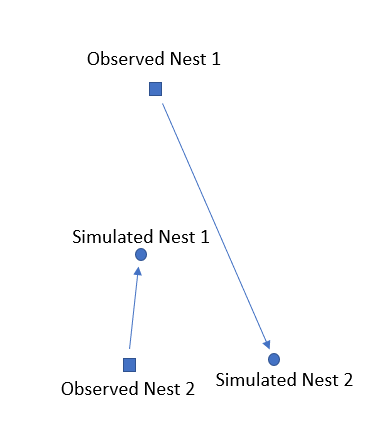
\includegraphics[width=0.3\linewidth]{subs1.PNG}}
 \subfloat[B]{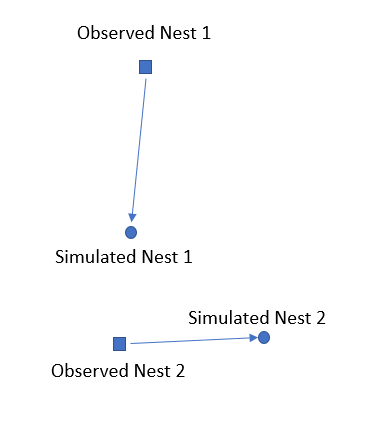
\includegraphics[width=0.3\linewidth]{subs2.PNG}}
\caption{[A] shows the shortest distance substitution in the deterministic scenario. [B] shows the more likely substitution that would be discarded in the deterministic scenario.}
\label{fig:1}
\end{figure*}

A better strategy is to assume that each set of particles that have been simulated up to time $T_i$ and have yet to be corrected can be corrected in a finite number of ways when we receive a new set of observation $\vec{z}^{\tau_i}$ at time $T_i$. We also make the assumption that once a particle have been corrected it will remain corrected in future times. These corrections are made with probability $H_{z^{\tau_i}}((\vec{s}^{T_i})' | \vec{s}^{T_i})_k$, where $(\vec{s}^{T_i})'$ is the vector of locations for the corrected nests at time $T_i$. Each time that a nest is corrected, its new location will correspond to the location of the observed nest that have caused the correction. If we have more simulated nests than what we have observed some nests will not be corrected and we will add them to the set of nests that still need to be corrected when the following set of observations will arrive. If we have more observed nests than simulated one, all nests will be corrected and we will add the observed nests left over (the one that where not responsible for a correction) to the set of nests simulated and observed.

The probability $H_{z^{\tau_i}}((\vec{s}^{T_i})' | \vec{s}^{T_i})_k$ of the new configuration of nests $k$ will depend on the distances between the simulated nests and the observed nests in the following way. Let us consider a simulated nest $s_j$ and an observation $z_h$. Then $s_j$ can be corrected by $z_h$ with probability $p_{s_j z_h} = p(s_j \leftrightarrow z_h) = e^{-d_{s_j z_h}}$ where $d_{s_j z_h}$ is the Euclidean distance between $s_j$ and $z_h$. Notice that when the distance is $d_{s_j z_h} = 0$ the probability $p_{s_j z_h}$ is 1 and the observation coincide with the simulated nest. The unnormalised probability of a certain new configuration $k$ of nests will therefore be $p((\vec{s}^{T_i})')_k = \prod_{h = 1}^{m^{\tau_i}} (p_{s_j z_h})$ where we remember that the quantity $m^{\tau_i}$ is the number of nests observed in the time interval between set of observations $\tau_i$. Therefore the probability of that configuration will be $H_{z^{\tau_i}} = p((\vec{s}^T)')_k / \sum_k p((\vec{s}^T)')_k $ where the sum is over all the possible configurations. So, each set simulated particle that have not been corrected can be corrected in only a finite number of ways to produce an element of the non-empty finite set $O_{\vec{z}^{\tau_i}} (\vec{s}^{T_i})$ that contains all the allowed corrections. The correction is made selecting an element $(\vec{s}^{T_i})'$ from the set $O_{\vec{z}^{T_i}} (\vec{s}^T)$ with probability $H_{z^{\tau_i}}$.

The selected configuration for the corrections will also determine $T_i$ to be the time of observation for those nests that have been corrected. For example if a nests was simulated as unobserved at time $T_i$ we will correct also the time of observation to be $T_i$. 

NOTE TO SELF: Notice that the simulated time of observation does not have an impact in the calculation of the probability for the corrections. We could improve this step adding that perhaps?

NOTE TO SELF: The normalization constant in the calculation of $H_{z^{\tau_i}}$ should cancel out when normalising the weight. 

NOTE TO SELF: The quantity $H_{z'^{\tau_i}}$ (notice the primed for z) which is the correction we would have made have we first generated the corrected sample then corrected in light of the observation is 1 as the corrected nests and the observed nests will coincide. If we add corrections for the nests that are not going to be located exactly in the location of the observed nests this quantity will not be 1.
}

{\color{red}
\subsection{The calculation of the Weights} \label{subsec:weight}

In this section we will use Sequential Importance Sampling with an auxiliary variable to facilitate sampling a Bayesian model involving partially observed states.

We will want to approximate the posterior $p(\vec{A}^{T_i} | \vec{Z}^{T_i})$ by iterative sampling and obtain Monte Carlo estimates of position, time of founding and observation time for the nests generated during the invasion. 





}

{\color{red}
\section{Pseudocode}

\begin{algorithm}[H]
\caption{SIR with corrections for RIFA invasion}
 \begin{algorithmic}

 \State  \bf{Initialize:} \normalfont At time $T_i$ with $i = 1$
            
\begin{enumerate}
	\item For $j = 1, \dots , n$ with $n$ number of particles
	\begin{enumerate}
		\item Sample from the model location of nests, time of founding and time of observation $\vec{f}^1_j$, $\vec{t}^1_j$, $\vec{x}^1_j$, $\vec{y}^1_j$.
		\item Evaluate the importance weights up to a normalising constant:
		\[
		\tilde{w}^{1}_{j} = 1
		\]
	\end{enumerate}
	\item For $j = 1, \dots , n$ normalise the importance weights: 
	\[
	w^{1}_{j} = \frac{1}{n}
	\]
\end{enumerate}

 \State  \bf{Iterate:} \normalfont For $T_i$ with $i$ from 2 to $F$ with $F$ the number of sets of observations received.

\begin{enumerate}
	\item For $j = 1, \dots , n$
	\begin{enumerate}
  		\item Sample from the model location of nests, time of founding and time of observation and generate vectors .
		\item Correct every element of $\vec{x}^t_i$ in light of the data $\vec{z}^t$ to obtain new samples $(\vec{x'})^t_i$.
		\item Evaluate the weights up to a normalising constant using equation (\ref{eq:2}):
		\[
		\tilde{w}^{t}_{i} = \frac{q(\vec{(x')}^{t}_i| \vec{z}^{\tau{i-1}})}{q(\vec{x}^{t}_i | \vec{Z}^{t-1}) H_\vec{z}^{\tau}_i}
		\]
	\end{enumerate}
	\item For $i = 1, \dots , n$ normalise the importance weights:
	\[
	w^{t}_{i} = \frac{\tilde{w}^t_i}{\sum_{k=1}^{n}\tilde{w}^{t}_k}
	\]
	\item Perform resampling
	\begin{enumerate}
	    \item Draw $n$ particles from the current particle set with probabilities proportional to their weights. Replace the current particle set with the new $n$ particles.
	    \item Set $w^t_i=1/n$
	\end{enumerate}
\end{enumerate}
  
 \end{algorithmic}
\end{algorithm}

}



\begin{thebibliography}{99}

\bibitem{GISD} GGISD (Global Invasive Species Database) (2020) Species profile: Solenopsis invicta. [30-09-2020] http://www.iucngisd.org/gisd/speciesname/Solenopsis+invicta

\bibitem{Hawkes71} Hawkes A G (1971) Spectra of some self-exciting and mutually exciting point processes. \textit{Biometrika} 58(1): 83-90

\bibitem{Hawkes74} Hawkes A G, Oakes D (1974) A cluster Process Representation Of A Self-Exciting Point Process. \textit{Journal of Applied Probabilities} 11(3): 493-503

\bibitem{Keith} Keith J M, Spring D (2013) Agent-based Bayesian approach to monitoring the progress of invasive species eradication programs. \textit{Proceedings of the National Academyof Sciences} 110(33): 13428-13433

\bibitem{Jewell} Jewell C P, Kypraios T, Neal P (2009) Bayesian analysis for emerging infectious diseases. \textit{Bayesian Anal.} 4(3): 465-496

\bibitem{Lewis} Lewis P (1964) A Branching Poisson Process Model for the Analysis of Computer Failure Patterns. \textit{Journal of the Royal Statistical Society} 26(3): 398-456

\bibitem{Ogata} Ogata Y (1981) On Lewis' simulation method for point processes. \textit{IEEE Transactions on Information Theory} 27(1): 23-31

\bibitem{Reinhart} Reinhart A (2017) A review of self-exciting spatio-temporal point processes and their applications. \textit{ArXiv e-prints} 1708.02647v2

\bibitem{Royle} Royle J A, Kry M, Gautier R, Schmid H (2007) Hierarchical spatial models of abundance and occurrence from imperfect survey data. \textit{Ecological Monographs} 77(3):465-481

\bibitem{Shoenberg} Shoenberg F P, Brillinger R, Guttorp P (2014). Point Processes, Spatial Temporal. \textit{Encyclopedia of Environmetrics}

\bibitem{Suarez} Suarez A V, Holway A, Case T J (2000) Patterns of spread in biological invasions dominated by long-distance jump dispersal: Insights from Argentine ants. \textit{Proc Natl Acad Sci} 98(3): 1095-1100

\bibitem{Wang} Wang L, Xu Y, Zeng L, Lu Y (2019). Impact of the red imported fire ant Solenopsis invicta Buren on biodiversity in South China: A review. \textit{Journal of Integrative Agriculture} 18(4): 788-796

\bibitem{Wetterer} Wetterer J K (2013). Exotic spread of Solenopsis invicta Buren (Hymenoptera: Formicidae) beyond North America. \textit{Sociobiology} 60: 50-55

\bibitem{WylieMay16} Wylie R, Janssen-May S (2016). Invader  Red imported fire ant in Australia:  What if we lose the war?. \textit{Ecological Management & Restoration} 18(1): 32-44

\bibitem{Wylie2020} Wylie R (2020). Invader at the gate: The status of redimported fire ant in Australia and Asia. \textit{Ecological Research} 35(1): 6-16

\bibitem{Zhuang} Zhuang J, Ogata Y, Vere-Jones D (2004). Analyzing Earthquake Clustering Features by Using Stochastic Reconstruction. \textit{Journal of Geophysical Research: Solid Earth} 109(B05301)

\bibitem{Wu} Wu W, Hong T, Zeng L, Huang D L, Chileshe J M, Chen J T, Yi C D, Liu X Y, Lu D H (2014). Detection of Solenopsis invicta (Hymenoptera: Formicidae) nests using spectral data. \textit{Florida Entomologist} 97(3): 967-971

\end{thebibliography}


\end{document}
